\documentclass{article}

\usepackage{arxiv}

\usepackage[utf8]{inputenc} % allow utf-8 input
\usepackage[T1]{fontenc}    % use 8-bit T1 fonts
\usepackage{lmodern}        % https://github.com/rstudio/rticles/issues/343
\usepackage{hyperref}       % hyperlinks
\usepackage{url}            % simple URL typesetting
\usepackage{booktabs}       % professional-quality tables
\usepackage{amsfonts}       % blackboard math symbols
\usepackage{nicefrac}       % compact symbols for 1/2, etc.
\usepackage{microtype}      % microtypography
\usepackage{graphicx}

\title{A template for the \emph{arxiv} style}

\author{
    H.Sherry Zhang
   \\
    Department of Econometrics and Business Statistics \\
    Monash University \\
  Melbourne, Australia \\
  \texttt{\href{mailto:huize.zhang@monash.edu}{\nolinkurl{huize.zhang@monash.edu}}} \\
   \And
    Dianne Cook
   \\
    Department of Econometrics and Business Statistics \\
    Monash University \\
  Melbourne, Australia \\
  \texttt{\href{mailto:dicook@monash.edu}{\nolinkurl{dicook@monash.edu}}} \\
   \And
    Ursula Laa
   \\
    Institute of Statistics \\
    University of Natural Resources and Life Sciences \\
  Vienna, Austria \\
  \texttt{\href{mailto:ursula.laa@boku.ac.at}{\nolinkurl{ursula.laa@boku.ac.at}}} \\
   \And
    Nicolas Langrené
   \\
    34 Village Street, Docklands VIC 3008 Australia \\
    CSIRO Data61 \\
  Melbourne, Australia \\
  \texttt{\href{mailto:nicolas.langrene@csiro.au}{\nolinkurl{nicolas.langrene@csiro.au}}} \\
   \And
    Patricia Menéndez
   \\
    Department of Econometrics and Business Statistics \\
    Monash University \\
  Melbourne, Australia \\
  \texttt{\href{mailto:patricia.menendez@monash.edu}{\nolinkurl{patricia.menendez@monash.edu}}} \\
  }

\usepackage{color}
\usepackage{fancyvrb}
\newcommand{\VerbBar}{|}
\newcommand{\VERB}{\Verb[commandchars=\\\{\}]}
\DefineVerbatimEnvironment{Highlighting}{Verbatim}{commandchars=\\\{\}}
% Add ',fontsize=\small' for more characters per line
\usepackage{framed}
\definecolor{shadecolor}{RGB}{248,248,248}
\newenvironment{Shaded}{\begin{snugshade}}{\end{snugshade}}
\newcommand{\AlertTok}[1]{\textcolor[rgb]{0.94,0.16,0.16}{#1}}
\newcommand{\AnnotationTok}[1]{\textcolor[rgb]{0.56,0.35,0.01}{\textbf{\textit{#1}}}}
\newcommand{\AttributeTok}[1]{\textcolor[rgb]{0.77,0.63,0.00}{#1}}
\newcommand{\BaseNTok}[1]{\textcolor[rgb]{0.00,0.00,0.81}{#1}}
\newcommand{\BuiltInTok}[1]{#1}
\newcommand{\CharTok}[1]{\textcolor[rgb]{0.31,0.60,0.02}{#1}}
\newcommand{\CommentTok}[1]{\textcolor[rgb]{0.56,0.35,0.01}{\textit{#1}}}
\newcommand{\CommentVarTok}[1]{\textcolor[rgb]{0.56,0.35,0.01}{\textbf{\textit{#1}}}}
\newcommand{\ConstantTok}[1]{\textcolor[rgb]{0.00,0.00,0.00}{#1}}
\newcommand{\ControlFlowTok}[1]{\textcolor[rgb]{0.13,0.29,0.53}{\textbf{#1}}}
\newcommand{\DataTypeTok}[1]{\textcolor[rgb]{0.13,0.29,0.53}{#1}}
\newcommand{\DecValTok}[1]{\textcolor[rgb]{0.00,0.00,0.81}{#1}}
\newcommand{\DocumentationTok}[1]{\textcolor[rgb]{0.56,0.35,0.01}{\textbf{\textit{#1}}}}
\newcommand{\ErrorTok}[1]{\textcolor[rgb]{0.64,0.00,0.00}{\textbf{#1}}}
\newcommand{\ExtensionTok}[1]{#1}
\newcommand{\FloatTok}[1]{\textcolor[rgb]{0.00,0.00,0.81}{#1}}
\newcommand{\FunctionTok}[1]{\textcolor[rgb]{0.00,0.00,0.00}{#1}}
\newcommand{\ImportTok}[1]{#1}
\newcommand{\InformationTok}[1]{\textcolor[rgb]{0.56,0.35,0.01}{\textbf{\textit{#1}}}}
\newcommand{\KeywordTok}[1]{\textcolor[rgb]{0.13,0.29,0.53}{\textbf{#1}}}
\newcommand{\NormalTok}[1]{#1}
\newcommand{\OperatorTok}[1]{\textcolor[rgb]{0.81,0.36,0.00}{\textbf{#1}}}
\newcommand{\OtherTok}[1]{\textcolor[rgb]{0.56,0.35,0.01}{#1}}
\newcommand{\PreprocessorTok}[1]{\textcolor[rgb]{0.56,0.35,0.01}{\textit{#1}}}
\newcommand{\RegionMarkerTok}[1]{#1}
\newcommand{\SpecialCharTok}[1]{\textcolor[rgb]{0.00,0.00,0.00}{#1}}
\newcommand{\SpecialStringTok}[1]{\textcolor[rgb]{0.31,0.60,0.02}{#1}}
\newcommand{\StringTok}[1]{\textcolor[rgb]{0.31,0.60,0.02}{#1}}
\newcommand{\VariableTok}[1]{\textcolor[rgb]{0.00,0.00,0.00}{#1}}
\newcommand{\VerbatimStringTok}[1]{\textcolor[rgb]{0.31,0.60,0.02}{#1}}
\newcommand{\WarningTok}[1]{\textcolor[rgb]{0.56,0.35,0.01}{\textbf{\textit{#1}}}}


% Pandoc citation processing
\newlength{\csllabelwidth}
\setlength{\csllabelwidth}{3em}
\newlength{\cslhangindent}
\setlength{\cslhangindent}{1.5em}
% for Pandoc 2.8 to 2.10.1
\newenvironment{cslreferences}%
  {}%
  {\par}
% For Pandoc 2.11+
\newenvironment{CSLReferences}[2] % #1 hanging-ident, #2 entry spacing
 {% don't indent paragraphs
  \setlength{\parindent}{0pt}
  % turn on hanging indent if param 1 is 1
  \ifodd #1 \everypar{\setlength{\hangindent}{\cslhangindent}}\ignorespaces\fi
  % set entry spacing
  \ifnum #2 > 0
  \setlength{\parskip}{#2\baselineskip}
  \fi
 }%
 {}
\usepackage{calc} % for calculating minipage widths
\newcommand{\CSLBlock}[1]{#1\hfill\break}
\newcommand{\CSLLeftMargin}[1]{\parbox[t]{\csllabelwidth}{#1}}
\newcommand{\CSLRightInline}[1]{\parbox[t]{\linewidth - \csllabelwidth}{#1}\break}
\newcommand{\CSLIndent}[1]{\hspace{\cslhangindent}#1}



\begin{document}
\maketitle

\def\tightlist{}


\begin{abstract}
Enter the text of your abstract here.
\end{abstract}

\keywords{
    blah
   \and
    blee
   \and
    bloo
   \and
    these are optional and can be removed
  }

\hypertarget{introduction}{%
\section{Introduction}\label{introduction}}

Spatio-temporal data record changes of variables in spatially separated
regions across time. In this article, we consider spatio-temporal vector
data, which are recorded in a fixed interval and are point based,
characterised by longitude and latitude, in the spatial aspect. Examples
of this type of data include the house price of a city or county,
climate measures from weather stations in a country, and river level
data from electronic gauges.

Analysing this type of data requires less considerations on the
geographical geometry type and map projection but more on how measures
in these fixed locations changes across the time domain and whether
these changes are related for adjacent locations. For example, when
nearby areas show patterns that are regular enough, visualising
spatio-temporal data can 1) discover regional time series features,
i.e.~trend and seasonality, 2) find the Waldo sites from the crowd, and
3) see how correlation of nearby sites changes across time.

The main difficulty in visualising this type of data is to show
information in both space and time dimension with the proper level of
details without information overflow. This would sometimes require
aggregating the time dimension into the proper level or slicing the data
into a reasonable number of subset for display. In this sense, a data
structure that regulates the manipulation spatio-temporal data will
benefit the analysis workflow. While many implementations focus on
manipulating and visualising pure spatial or temporal data, there are
not sufficient tools to deal with spatio-temporal data. The purpose of
this paper is to introduce a spatio-temporal vector data structure for
data analysis in R.

The rest of the paper will be divided as follows: Section 2 reviews the
existing data structure for spatio, temporal, and spatio-temporal data.
Section 3 presents a new data structure for spatio-temporal data:
cubble. Then the paper introduces the workflow of data manipulation and
visualisation with the cubble structure in Section 4. Section 5 gives
some examples on how common spatial and temporal manipulations are
performed with cubble and how static and interactive visualisation help
to understand climate and {[}\ldots{]} data.

\hypertarget{existing-data-structure-for-spatio-and-temporal-data}{%
\section{Existing data structure for spatio and temporal
data}\label{existing-data-structure-for-spatio-and-temporal-data}}

Below we review some structure for spatial, temporal, and
spatio-temporal data.

Many spatial and spatio-temporal data structures have been developed by
the R-spatial team for both raster and vector spatial data. For vector
spatial data, which is the focus of this paper, \texttt{sf} (E. J.
Pebesma 2018) represents spatial vector information with simple
features: points, lines, polygons and their multiples. Various
\texttt{st\_} function are designed to manipulate these features based
on their geometric relationships. For spatio-temporal data,
\texttt{stars} (E. Pebesma 2021) can represent both raster and vector
data using multi-dimensional array. However, the underlying array
structure can be difficult to operate for data analysts who are more
familiar with a flat 2D data frame structure used by the tidyverse
ecosystem.

In the temporal aspect, the \texttt{tsibble} (Wang, Cook, and Hyndman
2020) structure and its tidyverts ecosystem have provided a {[}\ldots{}
{]} workflow to work with temporal data. In a tsibble structure,
temporal data is characterised by \texttt{index} and \texttt{key} where
\texttt{index} is the temporal identifier and \texttt{key} is the
identifier for multiple series, which could be used as a spatio
identifier. However, a tsibble object, by construction, always requires
the \texttt{index} in its structure. This makes it less appealing for
spatio-temporal data since the output of calculated spatio-specific
variables (i.e.~features of each series) don't have the time dimension.
Analysts will either need to have an additional step to join this output
to the original tsibble or operate with variables stored in two separate
objects. In addition, the long form structure of a tsibble object means
spatio variables (i.e.~longitude, latitude, and features of each series
if joined back to the tsibble) of each spatio identifier will be
repetitively recorded at each timestamp. This repetition is unnecessary
and would inflate the object size for long series.

\hypertarget{a-new-data-structure-for-spatio-temporal-data}{%
\section{A new data structure for spatio-temporal
data}\label{a-new-data-structure-for-spatio-temporal-data}}

Spatio-temporal data can be thought of as characterised by three
dimensions: group, time, and variable, which allows us to use a cube to
represent the data. While group and time are can be seen as identifiers
of the record, variables can be further divided into those that are
group-related and time-related. Group-related variables are invariant to
the time and have only one value per group while time-related variables
change in time and requires both group and time to identify a record.
Hence the cubic representation can be further simplified for those
group-related variables as in the sketch \ref{fig:framework}, where
group-related variables are squashed in the time dimension.

\begin{figure}
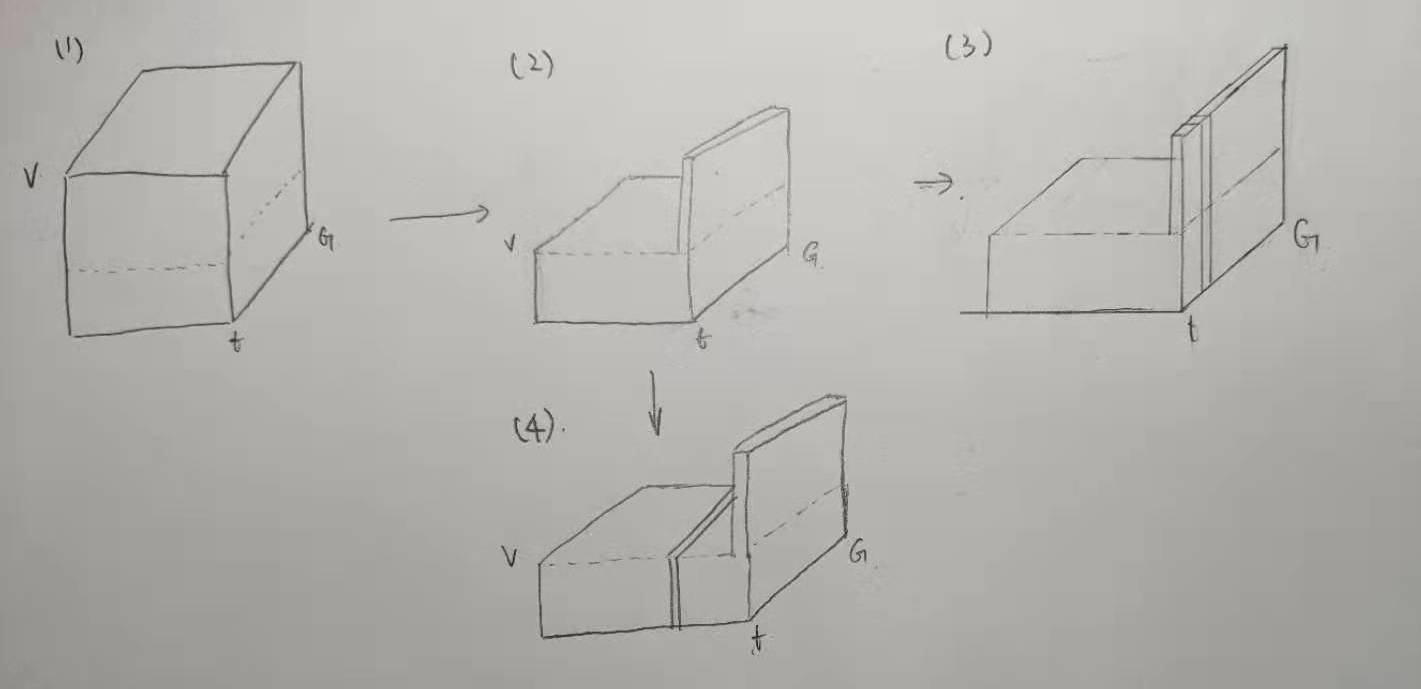
\includegraphics[width=1\linewidth,height=0.3\textheight]{/Users/hzha400/Documents/PhD/research/paper-cubble/figures/cubble-framework-hand} \caption{Cubic representation of spatio-temporal data. (1) shows the full cube, (2) simplifies teh cube by squashing the time dimension of time-invariant variables. With (2), a slice along the group dimension will affect both time-variant and invariant variables as in (3) while, a slice along the time will only affect the tim-variant variables as in (4).}\label{fig:framework}
\end{figure}

A cubble simplifies the workflow in spatio-temporal data through
managing group and time-related variables separately in two forms:
list-column and long form. The nested form:

\begin{itemize}
\tightlist
\item
  defines each group in a row,
\item
  displays the group-related variables in columns, and
\item
  nests all the time-related variables into a column called \texttt{ts}.
\end{itemize}

This form focuses on the time-invariant variable by squashing the time
dimension

In the long form,

\begin{itemize}
\tightlist
\item
  each combination of group and timestamp occupies a row
\item
  time-related variables are displayed, and
\item
  group-related variables are not explicitly displayed but can be
  accessed through the \texttt{meta} attribute
\end{itemize}

Below are the how the nested and long form look like for Australia
climate data, which records daily precipitation, maximum and minimum
temperature for 55 stations across Australia from 2015- 2020. Notice
that each station forms a group in both forms and specifically, the
nested and long form have a underlying \texttt{rowwise\_df} and
\texttt{grouped\_df} respectively.

\begin{verbatim}
## # Cubble: station-wise: nested form
## # Group:  station [55]
##    station       lat  long elevation name                ts                  
##    <fct>       <dbl> <dbl>     <dbl> <fct>               <list>              
##  1 ASN00001019 -14.3  127.      23   kalumburu           <tbl_ts [2,147 x 4]>
##  2 ASN00002012 -18.2  128.     422   halls creek airport <tbl_ts [2,191 x 4]>
##  3 ASN00003003 -17.9  122.       7.4 broome airport      <tbl_ts [2,192 x 4]>
##  4 ASN00006011 -24.9  114.       4   carnarvon airport   <tbl_ts [2,192 x 4]>
##  5 ASN00009021 -31.9  116.      15.4 perth airport       <tbl_ts [2,192 x 4]>
##  6 ASN00009193 -32.0  116.      43.1 rottnest island     <tbl_ts [2,192 x 4]>
##  7 ASN00009518 -34.4  115.      13   cape leeuwin        <tbl_ts [2,184 x 4]>
##  8 ASN00009789 -33.8  122.      25   esperance           <tbl_ts [2,187 x 4]>
##  9 ASN00010286 -31.6  117.     217.  cunderdin airfield  <tbl_ts [2,190 x 4]>
## 10 ASN00010917 -32.7  117.     275   wandering           <tbl_ts [2,192 x 4]>
## # ... with 45 more rows
\end{verbatim}

\begin{verbatim}
## # Cubble: time-wise: long form [tsibble]
## # Group:  station [55]
##    station     date        prcp  tmax  tmin
##    <fct>       <date>     <dbl> <dbl> <dbl>
##  1 ASN00001019 2015-01-01   164  31.5  25  
##  2 ASN00001019 2015-01-02   124  31.3  25  
##  3 ASN00001019 2015-01-03    50  29.2  24.7
##  4 ASN00001019 2015-01-04   204  32.1  24.3
##  5 ASN00001019 2015-01-05   412  31.4  24.6
##  6 ASN00001019 2015-01-06   200  28.7  25.1
##  7 ASN00001019 2015-01-07   822  30.2  24.5
##  8 ASN00001019 2015-01-08    22  31    26.6
##  9 ASN00001019 2015-01-09    62  32.7  26.2
## 10 ASN00001019 2015-01-10   274  32.9  22.6
## # ... with 120,311 more rows
\end{verbatim}

With a cubic framework on mind, different types of manipulation with
cubble can be thought of as slicing the cube in various way. The table
below shows how some \texttt{dplyr} verbs are mapped into the operation
in a cubble. With the existing grouping on the station, additional
groupping can be added with \texttt{group\_by} and removed with
\texttt{ungrouped}. {[}talk about why it is useful{]}

\begin{figure}
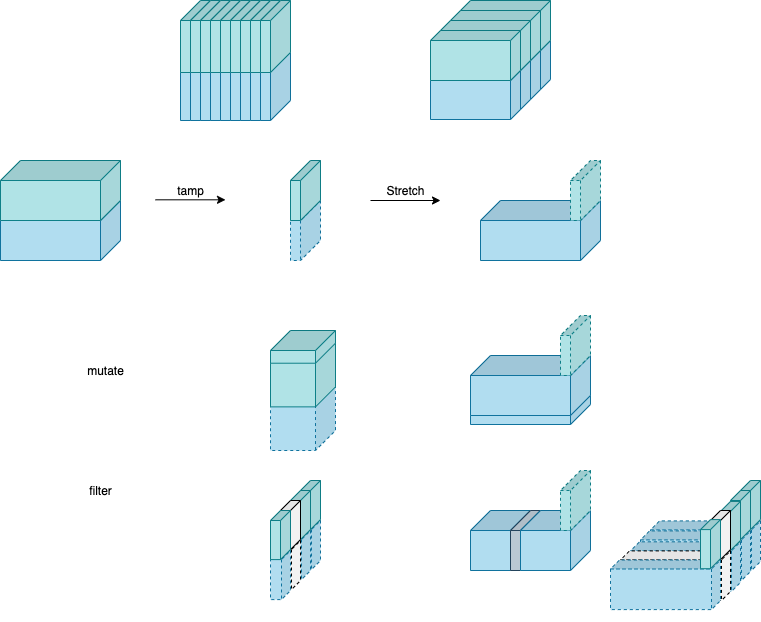
\includegraphics[width=1\linewidth,height=0.5\textheight]{/Users/hzha400/Documents/PhD/research/paper-cubble/figures/cubble-verbs} \caption{sdfsdf}\label{fig:verbs}
\end{figure}

\hypertarget{cubble-verbs}{%
\subsection{Cubble verbs}\label{cubble-verbs}}

Mention different types of manipulation with cubble:

\begin{itemize}
\tightlist
\item
  \texttt{dplyr} support for cubble:

  \begin{itemize}
  \tightlist
  \item
    basic 5s: mutate, filter, summarise, select, arrange
  \item
    group and ungroup: group\_by, ungroup
  \item
    slice family
  \end{itemize}
\item
  summarise missing stats
\end{itemize}

\newpage

\hypertarget{examples}{%
\section{Examples}\label{examples}}

Daily climate data (prcp, tmax, and tmin) from RNOAA - lots of stations
across Australia

An exploratory data analysis questions: What's the climate profile look
like in Australia

\begin{itemize}
\tightlist
\item
  General features: Any general trend/ fluctuation in prcp, tmax, and
  tmin?
\item
  Local features: Any station stands out from the crowd?
\end{itemize}

\hypertarget{manipulation}{%
\subsection{Manipulation}\label{manipulation}}

\hypertarget{mutate-and-filter}{%
\subsubsection{Mutate and filter}\label{mutate-and-filter}}

In the first example, we want to only keep the stations that have
\texttt{tmax} recorded in 2020. This requires first narrow down the
records to those in 2020, determine if \texttt{tmax} is missing for each
station, and then retain those stations that have \texttt{tmax}
recorded. The year filtering is an operation on the time axis, so we
start with the long form. Whether each station has \texttt{tmax}
recorded is a result of each station, rather than of each time point,
hence we need to switch to the nested form with \texttt{tamp()}. To
calculate whether \texttt{tmax} is recorded, we mutate a column
\texttt{tmax\_missing} that takes \texttt{TRUE} if all the \texttt{tmax}
in the nested list column \texttt{ts} are \texttt{NA} and \texttt{FALSE}
otherwise. To get the stations that we want, we need another filter on
\texttt{tmax\_missing}.

\begin{Shaded}
\begin{Highlighting}[]
\NormalTok{climate\_small }\SpecialCharTok{\%\textgreater{}\%} 
  \FunctionTok{stretch}\NormalTok{() }\SpecialCharTok{\%\textgreater{}\%} 
  \FunctionTok{filter}\NormalTok{(}\FunctionTok{year}\NormalTok{(date) }\SpecialCharTok{==} \DecValTok{2020}\NormalTok{) }\SpecialCharTok{\%\textgreater{}\%} 
  \FunctionTok{tamp}\NormalTok{() }\SpecialCharTok{\%\textgreater{}\%} 
  \FunctionTok{mutate}\NormalTok{(}\AttributeTok{tmax\_missing =} \FunctionTok{ifelse}\NormalTok{(}\FunctionTok{all}\NormalTok{(}\FunctionTok{is.na}\NormalTok{(ts}\SpecialCharTok{$}\NormalTok{tmax)), }\ConstantTok{TRUE}\NormalTok{, }\ConstantTok{FALSE}\NormalTok{)) }\SpecialCharTok{\%\textgreater{}\%} 
  \FunctionTok{filter}\NormalTok{(}\SpecialCharTok{!}\NormalTok{tmax\_missing)}
\end{Highlighting}
\end{Shaded}

\begin{verbatim}
## # Cubble: station-wise: nested form
## # Group:  station [55]
##    station      lat  long elevation name             ts             tmax_missing
##    <fct>      <dbl> <dbl>     <dbl> <fct>            <list>         <lgl>       
##  1 ASN000010~ -14.3  127.      23   kalumburu        <tbl_ts [366 ~ FALSE       
##  2 ASN000020~ -18.2  128.     422   halls creek air~ <tbl_ts [366 ~ FALSE       
##  3 ASN000030~ -17.9  122.       7.4 broome airport   <tbl_ts [366 ~ FALSE       
##  4 ASN000060~ -24.9  114.       4   carnarvon airpo~ <tbl_ts [366 ~ FALSE       
##  5 ASN000090~ -31.9  116.      15.4 perth airport    <tbl_ts [366 ~ FALSE       
##  6 ASN000091~ -32.0  116.      43.1 rottnest island  <tbl_ts [366 ~ FALSE       
##  7 ASN000095~ -34.4  115.      13   cape leeuwin     <tbl_ts [366 ~ FALSE       
##  8 ASN000097~ -33.8  122.      25   esperance        <tbl_ts [361 ~ FALSE       
##  9 ASN000102~ -31.6  117.     217.  cunderdin airfi~ <tbl_ts [366 ~ FALSE       
## 10 ASN000109~ -32.7  117.     275   wandering        <tbl_ts [366 ~ FALSE       
## # ... with 45 more rows
\end{verbatim}

\hypertarget{join}{%
\subsubsection{Join}\label{join}}

Now we want to select the stations that have been registered with world
meteorological organisation (WMO) and the dataset \texttt{station} has a
column \texttt{wmo\_id} that records this information. To do this task,
we first need to join the \texttt{station} dataset with our climate
dataset and then filter out those stations that don't have the WMO id.
Since the join is by station rather than by time, we start with the
nested form and write the exact same syntax of join and filter as with
tidyverse.

\begin{Shaded}
\begin{Highlighting}[]
\CommentTok{\# join wmo\_id for each station}
\NormalTok{to\_join }\OtherTok{\textless{}{-}}\NormalTok{ station }\SpecialCharTok{\%\textgreater{}\%} \FunctionTok{select}\NormalTok{(id, wmo\_id)}
\NormalTok{out }\OtherTok{\textless{}{-}}\NormalTok{ climate\_small }\SpecialCharTok{\%\textgreater{}\%} 
  \FunctionTok{left\_join}\NormalTok{(to\_join, }\AttributeTok{by =} \FunctionTok{c}\NormalTok{(}\StringTok{"station"} \OtherTok{=} \StringTok{"id"}\NormalTok{)) }\SpecialCharTok{\%\textgreater{}\%} 
  \FunctionTok{filter}\NormalTok{(}\SpecialCharTok{!}\FunctionTok{is.na}\NormalTok{(wmo\_id))}
\NormalTok{out}
\end{Highlighting}
\end{Shaded}

\begin{verbatim}
## # Cubble: station-wise: nested form
## # Group:  station [51]
##    station       lat  long elevation name              ts                 wmo_id
##    <fct>       <dbl> <dbl>     <dbl> <fct>             <list>              <dbl>
##  1 ASN00001019 -14.3  127.      23   kalumburu         <tbl_ts [2,147 x ~  94100
##  2 ASN00002012 -18.2  128.     422   halls creek airp~ <tbl_ts [2,191 x ~  94212
##  3 ASN00003003 -17.9  122.       7.4 broome airport    <tbl_ts [2,192 x ~  94203
##  4 ASN00006011 -24.9  114.       4   carnarvon airport <tbl_ts [2,192 x ~  94300
##  5 ASN00009021 -31.9  116.      15.4 perth airport     <tbl_ts [2,192 x ~  94610
##  6 ASN00009193 -32.0  116.      43.1 rottnest island   <tbl_ts [2,192 x ~  94602
##  7 ASN00009518 -34.4  115.      13   cape leeuwin      <tbl_ts [2,184 x ~  94601
##  8 ASN00009789 -33.8  122.      25   esperance         <tbl_ts [2,187 x ~  94638
##  9 ASN00010286 -31.6  117.     217.  cunderdin airfie~ <tbl_ts [2,190 x ~  95625
## 10 ASN00010917 -32.7  117.     275   wandering         <tbl_ts [2,192 x ~  95640
## # ... with 41 more rows
\end{verbatim}

Sometimes, we would like to have station-wise and time-wise variables in
the same form (i.e.~when plotting glyph maps). This can also be seen as
a joining task, on the long form, with the dataset to join being the
metadata. \texttt{migrate()} is a verb introduced as the shortcut for
\texttt{left\_join()} with a cubble's metadata and below is the
comparison of the two syntaxes.

\begin{Shaded}
\begin{Highlighting}[]
\NormalTok{out }\SpecialCharTok{\%\textgreater{}\%} 
  \FunctionTok{stretch}\NormalTok{() }\SpecialCharTok{\%\textgreater{}\%} 
  \FunctionTok{migrate}\NormalTok{(station, lat, long)}
\end{Highlighting}
\end{Shaded}

\begin{verbatim}
## # Cubble: time-wise: long form
## # Group:  station [55]
##    station     date        prcp  tmax  tmin   lat  long
##    <fct>       <date>     <dbl> <dbl> <dbl> <dbl> <dbl>
##  1 ASN00001019 2015-01-01   164  31.5  25   -14.3  127.
##  2 ASN00001019 2015-01-02   124  31.3  25   -14.3  127.
##  3 ASN00001019 2015-01-03    50  29.2  24.7 -14.3  127.
##  4 ASN00001019 2015-01-04   204  32.1  24.3 -14.3  127.
##  5 ASN00001019 2015-01-05   412  31.4  24.6 -14.3  127.
##  6 ASN00001019 2015-01-06   200  28.7  25.1 -14.3  127.
##  7 ASN00001019 2015-01-07   822  30.2  24.5 -14.3  127.
##  8 ASN00001019 2015-01-08    22  31    26.6 -14.3  127.
##  9 ASN00001019 2015-01-09    62  32.7  26.2 -14.3  127.
## 10 ASN00001019 2015-01-10   274  32.9  22.6 -14.3  127.
## # ... with 111,562 more rows
\end{verbatim}

\begin{itemize}
\tightlist
\item
  data quality check: filter out stations have variables not properly
  recorded
\item
  data summary:

  \begin{itemize}
  \tightlist
  \item
    daily -\textgreater{} monthly/ weekly,
  \item
    summarise by mean for tmax/ tmin, sum for prcp
  \end{itemize}
\item
\end{itemize}

\hypertarget{graphics}{%
\subsection{Graphics}\label{graphics}}

Static + interactive -\textgreater{} tooltip to show additional
information upon hovering

\begin{itemize}
\tightlist
\item
  Where are those stations on the map?

  \begin{itemize}
  \tightlist
  \item
    Mention mostly aero, airport, and lighthouse
  \end{itemize}
\end{itemize}

\hypertarget{summary}{%
\section*{Summary}\label{summary}}
\addcontentsline{toc}{section}{Summary}

\hypertarget{refs}{}
\begin{CSLReferences}{1}{0}
\leavevmode\hypertarget{ref-stars}{}%
Pebesma, Edzer. 2021. \emph{Stars: Spatiotemporal Arrays, Raster and
Vector Data Cubes}. \url{https://CRAN.R-project.org/package=stars}.

\leavevmode\hypertarget{ref-pebesma2018simple}{}%
Pebesma, Edzer J. 2018. {``Simple Features for r: Standardized Support
for Spatial Vector Data.''} \emph{R J.} 10 (1): 439.

\leavevmode\hypertarget{ref-tsibbles}{}%
Wang, Earo, Dianne Cook, and Rob J Hyndman. 2020. {``A New Tidy Data
Structure to Support Exploration and Modeling of Temporal Data.''}
\emph{Journal of Computational and Graphical Statistics} 29 (3):
466--78. \url{https://doi.org/10.1080/10618600.2019.1695624}.

\end{CSLReferences}

\bibliographystyle{unsrt}
\bibliography{references.bib}


\end{document}
